%! Author = itgramic
%! Date = 05.12.23

% Preamble
\begin{flushleft}
    \subsubsection{yugabyteDB - Distributed SQL 101}
    yugabyteDB - Distributed SQL 101 ist eine nahezu komplett \Gls{PostgreSQL} Kompatible Datenbank.
    Sie ist eine Distributed SQL Datenbank, also eine Verteilte Datenbank\cite{ZXD6D9KU}.
\end{flushleft}
\begin{flushleft}
    \paragraph{Architektur}
    yugabyteDB ist kein reines \Gls{RDBMS}, resp. gar keines.
    Die Basis besteht aus einem \Gls{Key-Value-Store}.
    Darüber wurde eine \Gls{Cassandra}-like Query API und eine PostgreSQL like SQL API aufgebaut:
    \begin{figure}[H]
        \centering
        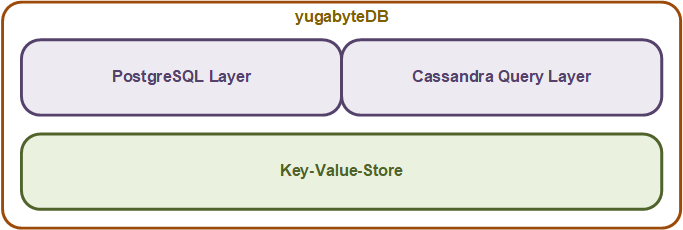
\includegraphics[width=0.8\linewidth]{source/implementation/evaluation/postgresql_ha_solutions/yugabytedb/yugabytedb-concept}
        \caption{yugabyteDB - Grundkonzept}
        \label{fig:yugabytedb-concept}
    \end{figure}

    Der Basisaufbau wiederum beinhaltet diverse Dienste für das Sharding, die Replikation und Transaktionen:
    \begin{figure}[H]
        \centering
        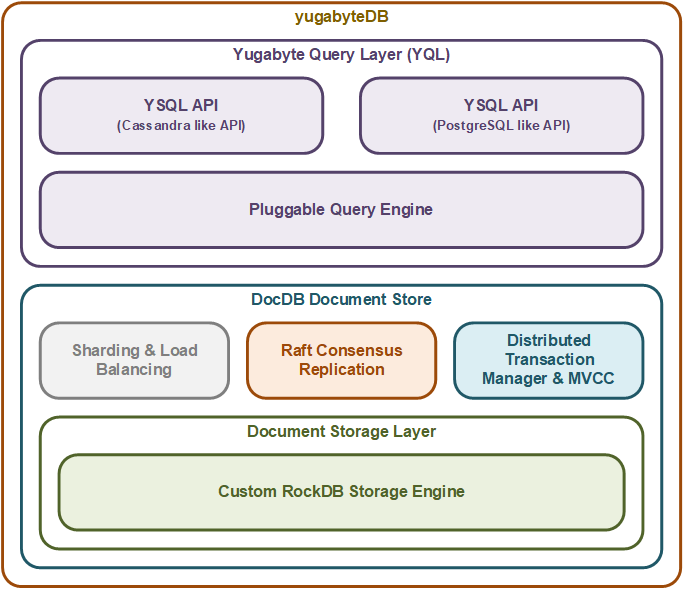
\includegraphics[width=0.8\linewidth]{source/implementation/evaluation/postgresql_ha_solutions/yugabytedb/yugabytedb-basic-archicture}
        \caption{yugabyteDB - Architektur}
        \label{fig:yugabytedb-basic-archicture}
    \end{figure}

    \subparagraph{yugabyteDB - Sharding}
    yugabyteDB teilt seine Tabellen in Tablets auf.
    Die Aufteilung kann gemäss Sharding-Standards gemacht werden:
    \begin{figure}[H]
        \centering
        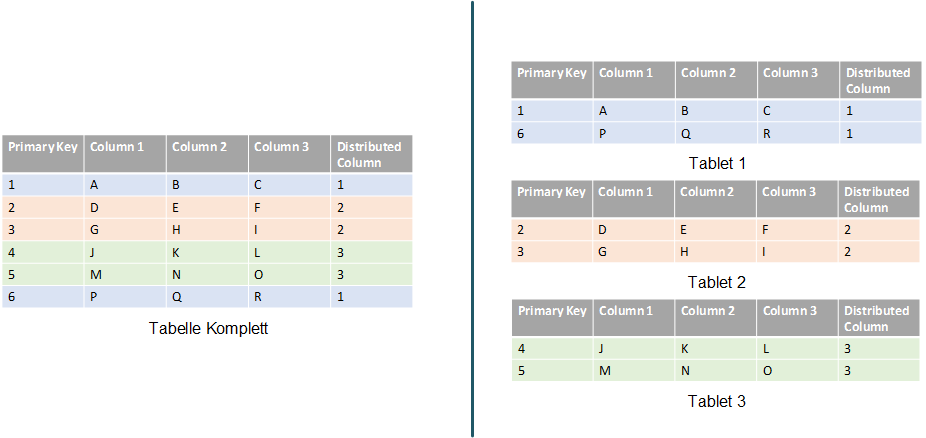
\includegraphics[width=0.8\linewidth]{source/implementation/evaluation/postgresql_ha_solutions/yugabytedb/yugabytedb-sharding-tablets}
        \caption{yugabyteDB - Sharding}
        \label{fig:yugabytedb-sharding-tablets}
    \end{figure}

    Dabei hat jedes Tablet auf einem Node einen Leader, der an die Follower auf den anderen Nodes repliziert:
    \begin{figure}[H]
        \centering
        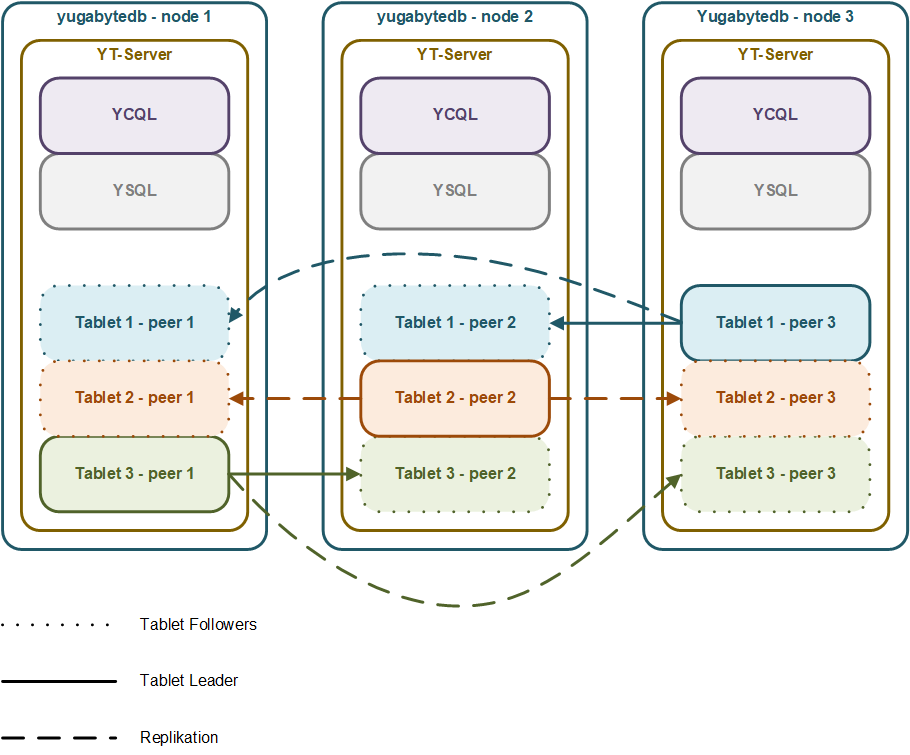
\includegraphics[width=0.8\linewidth]{source/implementation/evaluation/postgresql_ha_solutions/yugabytedb/yugabytedb-tablet-masters}
        \caption{yugabyteDB - Tablet - Leader und Follower}
        \label{fig:yugabytedb-tablet-masters}
    \end{figure}




\end{flushleft}

